% EEG-JEPA -- Hack the World(s), team Hello Worlds.
% LaTeX scaffold adapted from Tariolle/sls-wm/presentation (metropolis + TikZ).
\documentclass[aspectratio=169]{beamer}
\usetheme{metropolis}

\usepackage{booktabs}
\usepackage{colortbl} % \rowcolor
\usepackage{multirow}
\usepackage{amsmath}
\usepackage{graphicx}
\usepackage{hyperref}
\usepackage[normalem]{ulem} % for \sout (strikethrough)
\usepackage{tikz}
\usetikzlibrary{positioning, fit, arrows.meta, calc, decorations.pathreplacing, backgrounds}

\graphicspath{{./figures/}{../results/label_eff/}{../results/benchmark/}{../results/robustness/}{../results/calibration/}{../results/latent/}{../results/loss/}{../results/riemann/}{../}}

\definecolor{insared}{HTML}{E51F13}
\definecolor{vcolor}{HTML}{2E86AB}   % encoder / our method (blue)
\definecolor{mcolor}{HTML}{E8871E}   % regulariser / SSL (orange)
\definecolor{ccolor}{HTML}{7FB069}   % probe / eval (green)
\setbeamercolor{progress bar}{fg=normal text.fg}   % match the (dark blue) text colour
\setbeamertemplate{frame footer}{}
\metroset{block=fill}
% Reduce frame title spacing to prevent overflow
\addtobeamertemplate{frametitle}{}{\vspace*{-0.3em}}

% ---- Project constants: change here, propagates everywhere ----
\newcommand{\nchan}{19}                % EEG channels
\newcommand{\sfreq}{200}               % Hz
\newcommand{\winsec}{10}               % window length (s)
\newcommand{\winsamp}{2{,}000}         % samples per window (\winsec * \sfreq)
\newcommand{\dmodel}{256}              % encoder feature dim
\newcommand{\dcov}{32}                 % covariance projection dim (tangent arm)
\newcommand{\tprime}{125}              % time steps after 4 stride-2 blocks
\newcommand{\epochs}{30}               % SSL epochs
\newcommand{\batch}{256}               % SSL batch size
\newcommand{\ba}{0.819}                % 3-seed mean balanced accuracy
\newcommand{\babest}{0.833}            % best-seed balanced accuracy
\newcommand{\aurocv}{0.89}             % 3-seed mean AUROC (0.891; best seed 0.90) -- see results/benchmark/jepa_eval_seeds.json
\newcommand{\floorv}{0.79}             % random-init-encoder floor
\newcommand{\riem}{0.761}              % Riemannian 0-param yardstick
\newcommand{\nrectr}{2{,}717}          % train recordings
\newcommand{\nrecev}{276}              % eval recordings
\newcommand{\npattr}{2{,}076}          % train patients
\newcommand{\npatev}{253}              % eval patients

\title{Geometry-Aware JEPA for EEG}
\subtitle{A controlled frozen-transfer study on TUAB}
\author{Florent Tariolle \and Cl\'ement Genninasca \and Yoann Frayce \and Hippolyte du Pac de Marsoulies}
\institute{Hack the World(s) -- EEG Track \quad$\cdot$\quad Team \textbf{HelloWorlds}}
\date{}

% ============================================================
\begin{document}

% --- Title ---
{%
\setbeamertemplate{headline}{}
\begin{frame}[noframenumbering,plain]
  \titlepage
\end{frame}
}

% ==========================================================
\section{Contribution}
% ==========================================================

\begin{frame}{Our contribution, in one slide}
  \small
  \begin{enumerate}
    \item \textbf{A strong frozen baseline.} SIGReg-ambient JEPA matches the LeJEPA/Laya recipe's value on our setup -- not a controlled head-to-head.
    \item \textbf{Nothing beats it.} Ambient/tangent SIGReg \& PEIRA, Graph-JEPA, Fourier-JEPA -- none beats ambient SIGReg in balanced accuracy.
    \item \textbf{Latent geometry is the contribution.} Visualised with \textbf{de Surrel's AIRM Riemannian t-SNE} (the right metric for SPD/EEG covariances).
  \end{enumerate}
\end{frame}

% ==========================================================
\section{Motivation}
% ==========================================================

\begin{frame}{The question we actually asked}
  \vfill
  \begin{itemize}
    \item \textbf{EEG foundation models} are everywhere -- but most report \emph{fine-tuned} numbers. What survives when you \textbf{freeze} the encoder?
    \item \textbf{JEPA} avoids collapse with an \emph{anti-collapse regulariser}. The EEG covariance lives on a curved \textbf{SPD manifold}, not in flat Euclidean space.
    \item \textbf{Our intuition}: a \emph{Riemannian geometry-aware} anti-collapse regulariser -- acting in the SPD \textbf{tangent} of the EEG covariance, not flat ambient space -- should \emph{respect and improve} the latent geometry.
    \item \textbf{What we ship}: a strong frozen probe \emph{and} a geometry-aware regulariser that \textbf{measurably sharpens the latent-space geometry}, visualised with de Surrel's AIRM Riemannian t-SNE.
  \end{itemize}
\end{frame}

% ==========================================================
\section{Data}
% ==========================================================

\begin{frame}{Data: TUH Abnormal EEG (TUAB)}
  \vspace{0.3em}
  \begin{itemize}
    \item \textbf{Task}: binary \emph{normal} vs \emph{abnormal} EEG, recording level.
    \item \textbf{Signal}: \nchan{} channels @ \sfreq~Hz; \winsec~s windows ($\winsamp$ samples).
    \item \textbf{Standard split}: \nrectr{} train / \nrecev{} eval recordings, \textbf{patient-disjoint}.
    \item \textbf{Pretraining}: SSL reads only \emph{unlabeled} train recordings.
  \end{itemize}
\end{frame}


% ==========================================================
\section{Architecture}
% ==========================================================

\begin{frame}{Two view and 1D convolutional encoder}
   \begin{center}
\vspace{0.3em}
  \resizebox{0.97\textwidth}{!}{%
  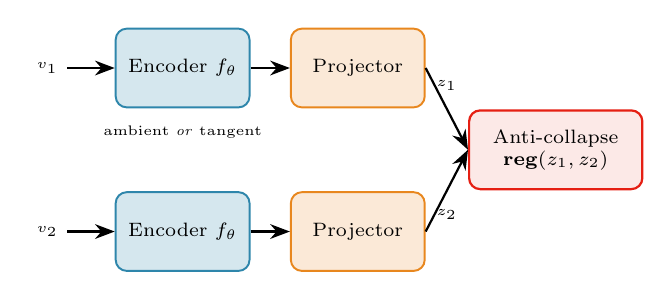
\begin{tikzpicture}[
    block/.style={rectangle, draw, rounded corners, minimum height=1.0cm, minimum width=1.7cm, align=center, font=\scriptsize, line width=0.7pt},
    reg/.style={rectangle, draw=insared, fill=insared!10, rounded corners, minimum height=1.0cm, minimum width=2.2cm, align=center, font=\scriptsize, line width=0.8pt},
    arr/.style={-{Stealth[length=2.5mm]}, thick},
    lbl/.style={font=\tiny, align=center},
  ]
    \node[lbl] (v1) {$v_1$};
    \node[lbl, below=1.7cm of v1] (v2) {$v_2$};
    \node[block, fill=vcolor!20, draw=vcolor, right=0.6cm of v1] (e1) {Encoder $f_\theta$};
    \node[block, fill=vcolor!20, draw=vcolor, right=0.6cm of v2] (e2) {Encoder $f_\theta$};
    \node[block, fill=mcolor!18, draw=mcolor, right=0.5cm of e1] (p1) {Projector};
    \node[block, fill=mcolor!18, draw=mcolor, right=0.5cm of e2] (p2) {Projector};
    \node[reg, right=1.4cm of $(p1)!0.5!(p2)$] (reg) {Anti-collapse\\\textbf{reg}$(z_1,z_2)$};
    \node[lbl, below=0.10cm of e1] {ambient \emph{or} tangent};

    \draw[arr] (v1) -- (e1);
    \draw[arr] (v2) -- (e2);
    \draw[arr] (e1) -- (p1);
    \draw[arr] (e2) -- (p2);
    \draw[arr] (p1.east) -- node[above=3pt,lbl]{$z_1$} (reg.west);
    \draw[arr] (p2.east) -- node[below=3pt,lbl]{$z_2$} (reg.west);
  \end{tikzpicture}%
  }
  \end{center}
\end{frame}

\begin{frame}{What we tried}
  \vspace{0.4em}
  \begin{center}
  \begin{tabular}{lcc}
    \toprule
    \textbf{regulariser} $\backslash$ \textbf{space} & \textbf{ambient} (Euclidean) & \textbf{tangent} (SPD) \\
    \midrule
    \textbf{VICReg} (variance/cov) & \texttt{C0} reference & --- \\
    \textbf{SIGReg} (Gaussianity slices) & \texttt{C1} \emph{Laya-like baseline} & \texttt{C2} geometry-aware \\
    \textbf{PEIRA} (distribution-free) & \texttt{C3} & \texttt{C4} \emph{ex-hypothesis} \\
    \bottomrule
  \end{tabular}
  \end{center}

  \vspace{0.8em}
  \begin{itemize}
    \item \textbf{SIGReg} (LeJEPA/BCS): tests random 1-D slices for Gaussianity -- assumes an \emph{isotropic} target.
    \item \textbf{PEIRA}: distribution-free anti-collapse -- no target distribution to mis-specify.
    \item \textbf{GraphJEPA}
    \item \textbf{FourierJEPA}
  \end{itemize}
\end{frame}


% ==========================================================
\section{Results}
% ==========================================================

\begin{frame}{SSL training curves (all cells healthy)}
  \vspace{-0.2em}
  \begin{center}
    
\includegraphics[width=\textwidth]{loss_curves.png}
  \end{center}
  \vspace{-0.4em}
  \begin{center}\footnotesize
    30 epochs, TUAB pretrain. All five cells converge and \textbf{none collapses} (eff.\ rank rises, feat.\ std ${\approx}1$). PEIRA satisfies anti-collapse \emph{harder} ($\sim3\times$ the eff.\ rank) yet wins nothing downstream -- collapse is not the binding constraint on TUAB. (Total loss is not comparable across objectives -- read per-curve shape.)
  \end{center}
\end{frame}

\begin{frame}{Frozen \& in-domain: we hold where frozen FMs fall}
  \vfill
  \begin{center}
    
\includegraphics[width=\textwidth]{frozen_headtohead.png}
  \end{center}
  \vfill
\end{frame}

\begin{frame}{Beyond accuracy: frozen-probe robustness (3-seed)}
  \vfill
  \vspace*{0.05\textheight}                                   % 5% lower
  \begin{center}
    
\includegraphics[width=1\textwidth]{robustness_3seed.png}
  \end{center}
  \vfill
  \vspace*{-0.05\textheight}
\end{frame}


% ==========================================================
\section{Visualization}
% ==========================================================



\begin{frame}{Manifold-aware latent geometry (AIRM vs Euclidean)}
  \vfill
  \vspace*{0.00\textheight}               
  \begin{center}
    
\includegraphics[width=\textwidth]{riemann_latent.png}      % bigger -- maxed to slide width
  \end{center}
  \vfill
  \vspace*{-0.05\textheight}
\end{frame}

\begin{frame}{Manifold viz generalises across sustained TUH tasks}
  \vfill
  \begin{center}
    
\includegraphics[width=\textwidth,height=0.9\textheight,keepaspectratio]{riemann_latent_tusz.png}
  \end{center}
  \vfill
\end{frame}




% ==========================================================
\section{Conclusion}
% ==========================================================

\begin{frame}{Conclusion}
  \vspace{0.8em}
  \begin{itemize}
    \item A \textbf{controlled frozen-transfer study}, not a leaderboard entry.
    \item \textbf{A strong frozen probe} (\ba{} BA, $\sim$\aurocv{} AUROC) that holds where published FMs collapse when frozen.
    \item \textbf{The payoff is the latent geometry}: a Riemannian geometry-aware (SPD-tangent) regulariser \textbf{sharpens the frozen latent} -- normal/abnormal and seizure classes form coherent structure -- and \textbf{de Surrel's AIRM Riemannian embedding sharpens it further over the Euclidean view}, most clearly for SIGReg.
    \item On this simple binary task the probe accuracy is the same across variants -- the tangent's gain is \emph{geometric}, exactly where a manifold-aware regulariser should help.
  \end{itemize}
  \vspace{1.0em}
  \begin{center}
    \large Built on a trimmed \texttt{eb\_jepa} vendor.
  \end{center}
\end{frame}

% ==========================================================
\section{References}
% ==========================================================

\begin{frame}[allowframebreaks]{References}
  \small
  \begin{itemize}
    % --- JEPA objective lineage (what we built on) ---
    \item Balestriero, R.\ \& LeCun, Y.\ (2025). \href{https://arxiv.org/abs/2511.08544}{\textit{LeJEPA: Provable and Scalable Self-Supervised Learning Without the Heuristics}}. Preprint. \emph{(SIGReg -- our anti-collapse objective)}
    \item Panchavati, S.\ et al.\ (2026). \href{https://arxiv.org/abs/2603.16281}{\textit{Laya: a LeJEPA approach to EEG via latent prediction over reconstruction}}. Preprint. \emph{(our ambient baseline)}
    \item Arbel, M., Terver, B.\ \& Ponce, J.\ (2026). \href{https://arxiv.org/abs/2605.17671}{\textit{PEIRA: Learning Predictive Encoders through Inter-View Regressor Alignment}}. Preprint.
    \item Bardes, A., Ponce, J.\ \& LeCun, Y.\ (2022). \href{https://arxiv.org/abs/2105.04906}{\textit{VICReg}}. ICLR.
    \item LeCun, Y.\ (2022). \textit{A Path Towards Autonomous Machine Intelligence (JEPA)}. OpenReview.
    % --- SPD / Riemannian geometry ---
    \item de Surrel, T., Lotte, F., Chevallier, S.\ \& Yger, F.\ (2025). \href{https://arxiv.org/abs/2502.01512}{\textit{Wrapped Gaussian on the manifold of Symmetric Positive Definite Matrices}}. Preprint.
    \item de Surrel, T.\ \textit{r\_tSNE\_in\_C} -- Riemannian t-SNE on SPD matrices (AIRM). \href{https://github.com/thibaultdesurrel/r_tSNE_in_C}{github.com/thibaultdesurrel/r\_tSNE\_in\_C}. \emph{(our manifold-aware latent viz)}
    \item Wang, Z.\ et al.\ (2025). \href{https://arxiv.org/abs/2501.08139}{\textit{EEG-ReMinD: Self-Supervised State Reconstruction-Primed Riemannian Dynamics}}. Preprint. \emph{(Riemannian SPD SSL; reconstruction, not JEPA)}
    \item Chen, M.\ et al.\ (2025). \href{https://arxiv.org/abs/2508.04956}{\textit{MENDR: Manifold Explainable Neural Data Representations}}. Preprint. \emph{(first Riemannian-SPD EEG FM; precedent for the geometry null)}
    \item Gemein, L.\ et al.\ (2020). \href{https://arxiv.org/abs/2002.05115}{\textit{Machine-learning-based diagnostics of EEG pathology}}. NeuroImage. \emph{(Riemannian baseline)}
    % --- EEG foundation models (frozen head-to-head) ---
    \item Jiang, W.-B.\ et al.\ (2024). \href{https://arxiv.org/abs/2405.18765}{\textit{LaBraM: Large Brain Model for EEG}}. ICLR.
    \item Wang, J.\ et al.\ (2024). \href{https://arxiv.org/abs/2412.07236}{\textit{CBraMod: Criss-Cross Brain Foundation Model}}. Preprint.
    \item Yang, C.\ et al.\ (2023). \href{https://arxiv.org/abs/2305.10351}{\textit{BIOT: Biosignal Transformer}}. NeurIPS.
    \item Wang, G.\ et al.\ (2024). \href{https://openreview.net/forum?id=lvS2b8CjG5}{\textit{EEGPT: Pretrained Transformer for Universal and Reliable Representation of EEG Signals}}. NeurIPS.
    \item Foumani, N.\ et al.\ (2024). \href{https://arxiv.org/abs/2402.17772}{\textit{EEG2Rep: Enhancing Self-supervised EEG Representation Through Informative Masked Inputs}}. KDD.
    \item Kostas, D., Aroca-Ouellette, S.\ \& Rudzicz, F.\ (2021). \href{https://arxiv.org/abs/2101.12037}{\textit{BENDR: Transformers \& Contrastive SSL for EEG}}. Front.\ Hum.\ Neurosci.
    \item Xiong, W.\ et al.\ (2026). \href{https://arxiv.org/abs/2508.17742}{\textit{EEG-FM-Bench: Systematic Evaluation \& Diagnostic Analyses of EEG Foundation Models}}. ICML. \emph{(source of our frozen FM head-to-head numbers)}
    % --- Dataset \& code ---
    \item Obeid, I.\ \& Picone, J.\ (2016). \href{https://doi.org/10.3389/fnins.2016.00196}{\textit{The Temple University Hospital EEG Data Corpus}}. Front.\ Neurosci.\ 10:196. \emph{(TUAB / TUSZ / TUEV)}
    \item \texttt{eb\_jepa} -- JEPA reference implementation, Meta AI / FAIR. \href{https://github.com/facebookresearch/eb_jepa}{github.com/facebookresearch/eb\_jepa}. \emph{(our trimmed code vendor)}
  \end{itemize}
\end{frame}

\end{document}
